
\section{Zbieżność metody i błędy rozwiązania}
\label{sec:zbieznosc_i_blad}

O zbieżności rozwiązania możemy wnioskować na podstawie funkcji kształtu. Pierwszym warunkiem jest tzw. warunek zgodności. Mówi on o tym, że funkcje kształtu muszą być ciągłe w przestrzeni elementów. Dla prostego przypadku dwóch elementów liniowych jednowymiarowych ciągłość funkcji ilustruje rysunek \ref{fig:zgodnosc}. 

\begin{figure}[h]
\centering
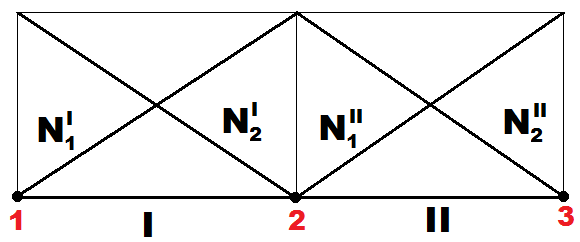
\includegraphics[width=10cm]{Zdjecia/3/zgodnosc}
\caption{Ciągłość funkcji w przestrzenii elementów}
\label{fig:zgodnosc}
\end{figure}

Warunek ten jest zapewniony poprzez własność funkcji kształtu przedstawioną we wzorze \ref{eq:eq_zgodnosc}.

Kolejny warunek nazywa się warunkiem bryły sztywnej (WBS). Zapewnia on brak straty bądź narastania energii podczas wyznaczania wyniku wewnątrz elementu. Warunek ten jest zapewniony poprzez własność funkcji kształtu przedstawioną w \ref{eq:WBS}.

Ostatnim warunkiem jest tzw. warunek stałego odkształcenia (WSO). Mówi on o tym, że jeśli w elemencie przyłożymy liniowe pole przemieszczeń, to odkształcenie będzie stałe w każdym punkcie elementu.

Jeśli spełnione są warunki zgodności, WBS oraz WBO to rozwiązanie dla elementu będzie zbieżne. Warunki te muszą być spełnione dla każdego elementu obliczanego modelu.

\vspace{3mm}

Zbieżność nie daje nam gwarancji, że rozwiązanie otrzymane przy pomocy symulacji MES jest poprawne. Przez poprawne rozumiane jest, że błąd rozwiązania jest dostatecznie mały. Aby mieć pewność, że rozwiązanie jest wystarczająco dokładne należy oszacować błąd maksymalny. W przypadku MES błąd powodują:

\begin{enumerate}
	\item dyskretyzacja konstrukcji 
	\item zaokrąglenia arytmetyczne.
\end{enumerate}

\vspace{3mm}

Pierwsza przyczyna występowania błędów związana jest z podziałem konstrukcji na elementy skończone. Błąd zawarty jest już w równaniu \( \textbf{M} \ddot{\textbf{x}} + \textbf{Kx} = \textbf{F} \). Pojawia się dlatego, że całe rozwiązanie wyznaczamy za pomocą wielomianowych funkcji kształtu. Błąd zbieżnego rozwiązania możemy zmniejszać poprzez wykorzystanie funkcji kształtu wyższego rzędu, bądź zagęszczenie siatki i budowę większej liczby elementów skończonych.

Estymacja błędów odbywa się na różne sposoby. Jednym z nich jest wykorzystanie równania \ref{eq:blad1}. 

\begin{equation} \label{eq:blad1}
	F - \tilde{F}_i \approx ch_i^r
\end{equation}

gdzie
\begin{eqwhere}[2cm]
	\item[$ F $] rozwiązanie dokładne
	\item[$ \tilde{F}_i $] i-te rozwiązanie przybliżone
	\item[$ c $] współczynnik proporcjonalności
	\item[$ h_i $] współczynnik zależny od zagęszczenia siatki
	\item[$ r $] współczynnik zależny od stopnia wielomianów interpolujących.
\end{eqwhere}

Jedna symulacja nie daje możliwości wyznaczyć błędu. Aby tego dokonać należy przeprowadzić dwie symulacje, co pozwala obliczyć błąd drugiej (dokładniejszej). Przyjmijmy, że druga symulacja zawiera elementy o dwukrotnie mniejszych wymiarach, czyli \( h_1 = 2h_2 \). Współczynnik \( r \) przyjmuje wartości mniejsze od 1, ale dla uproszczenia przyjmijmy dokładnie 1.

Podstawiając odpowiednie indeksy do wzoru \ref{eq:blad1}, możemy wyznaczyć błąd drugiej symulacji, znając wyniki zarówno pierwszej jak i drugiej.

\begin{equation} 
	F- \tilde{F}_2 \approx \frac{\tilde{F}_2 - \tilde{F}_1}{(\frac{h_1}{h_2})^r - 1}.
\end{equation}

\vspace{5mm}

Innym podejściem jest wyznaczanie błędów poprzez energię naprężenia elementów. Po wyznaczeniu przemieszczeń węzłów i obliczeniu naprężeń, naprężenia nie są ciągłe w przestrzeni elementów. Jeśli jeden węzeł należy do kilku elementów, to w każdym z nich może zostać wyznaczona inna wartość naprężenia dla takiego węzła. W ciągłym przypadku naprężenie byłoby funkcją ciągłą, dlatego błąd wynikający z naprężeń wyznacza się w następujący sposób:

\vspace{3mm}

\begin{enumerate}
	\item Obliczamy średnią naprężeń w węźle, biorąc wartości dla węzła z każdego elementu, do którego należy.
	\item Wyznaczamy błąd naprężenia w węzłach elementu, poprzez odejmowanie od naprężenia w węźle wartości średniego naprężenia w tym węźle.
	\item Sumujemy błędy naprężeń wszystkich elementów skończonych.
	\item Wyznaczamy energię błędu naprężenia.
	\item Wyznaczamy energię odkształcenia dla całej konstrukcji.s
	\item Obliczamy błąd procentowy według wzoru \ref{eq:blad2}.
\end{enumerate}

\vspace{3mm}

\begin{equation} \label{eq:blad2}
	E = 100(\frac{e}{U + e})^{0.5}
\end{equation}

gdzie
\begin{eqwhere}[2cm]
	\item[$ e $] całkowita energi błędu dla konstrukcji
	\item[$ U $] energi odkształcenia dla konstrukcji
	\item[$ E $] błąd procentowy energii.
\end{eqwhere}




















